\chapter{Background}
\label{cha:bg}

This chapter will cover some of the background material required for the following sections, it will cover the history of reinforcement learning (RL) and it's evolution to the current state-of-the-art. Additionally, it will cover the related work to this project and also cover some details of the past research papers for which this project has been based upon.

\section{Reinforcement learning}
\label{bg:sec:rl}
Reinforcement learning is an area of machine learning has has been under active research since the late 1980s (TODO: ref watkins phd). One of the earliest applications of RL is for the game of backgammon. TD-Gammon is a computer program developed by Gerald Tesauro in 1992 to play the game of backgammon using \textit{`temporal-difference learning'}.

\subsection{Deep reinforcement learning}
\label{bg:sec:deeprl}
Following from section \ref{bg:sec:rl} on RL, this section talks about the combination of two areas, deep learning and reinforcement learning methods, called deep reinforcement learning (DRL). Deep learning (DL) is a common class of machine learning methods that has been of much research focus over the past decade and can deal with high-dimensional sensory input; for the case of Atari this is 84x84x4 greyscale images after pre-processing of the raw Atari frames. On the other hand, reinforcement learning allows us to create an agent which can learn an optimal policy to navigate some environment in order to optimise its reward.

\begin{figure}[htbp]
	\centering
	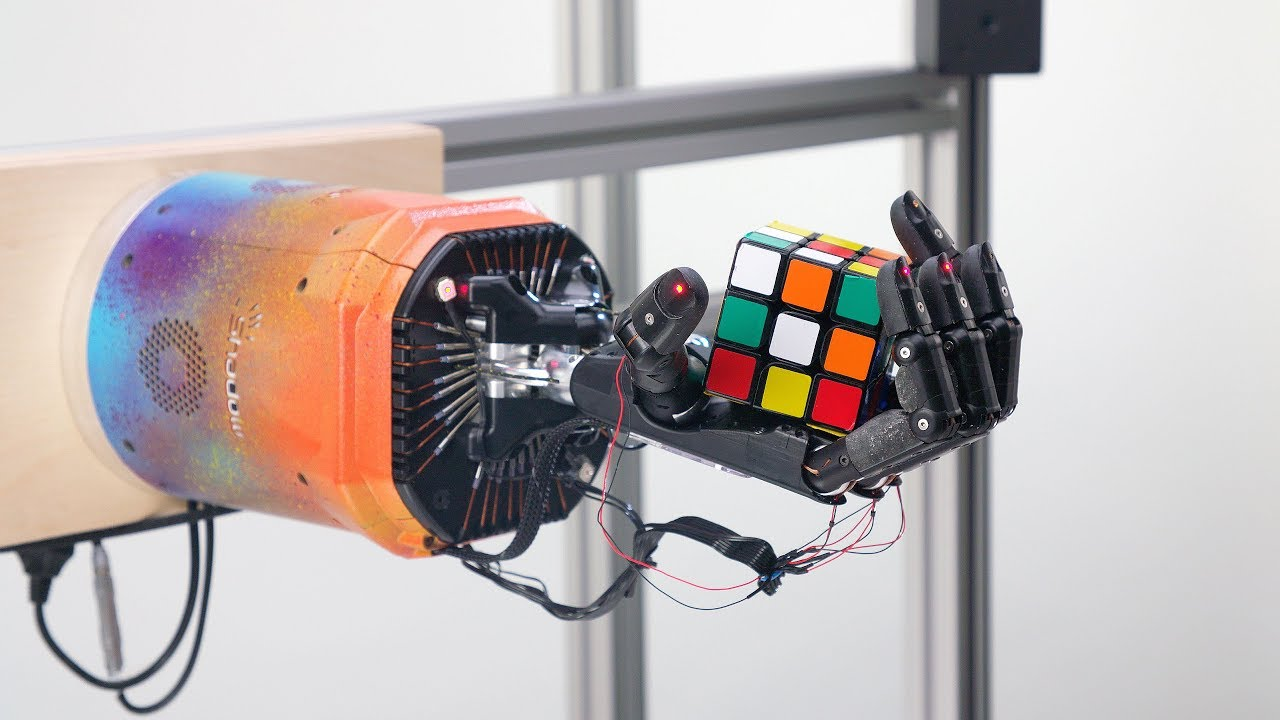
\includegraphics[width=0.5\textwidth]{chapters/chapter2/images/openai-robot.jpg}
	\caption{OpenAI Robot solving a Rubik's cube
		\label{fig:openai-robot}
	}
\end{figure}

Through the combination of these methods, it has proven to provide solutions to previously intractable problems \cite{rl-survey} in areas such as robotics, computer vision and healthcare. For example, in 2019 OpenAI developed a robotic hand that could solve a Rubik's cube \ref{fig:openai-robot}, trained using deep reinforcement learning. As an extension to DRL, end-to-end reinforcement learning is a method for single layered neural network, trained by reinforcement learning. Figure \ref{fig:e2e-rl} shows, diagramatically, how DL and RL are used together in order to produce a single end-to-end model. In this simple architcture, there are two main components, the agent and the environment. Throughout all DRL methods, this is common to see, an agent observes some state and reward from the environment after taking an action.

\begin{figure}[htbp]
	\centering
	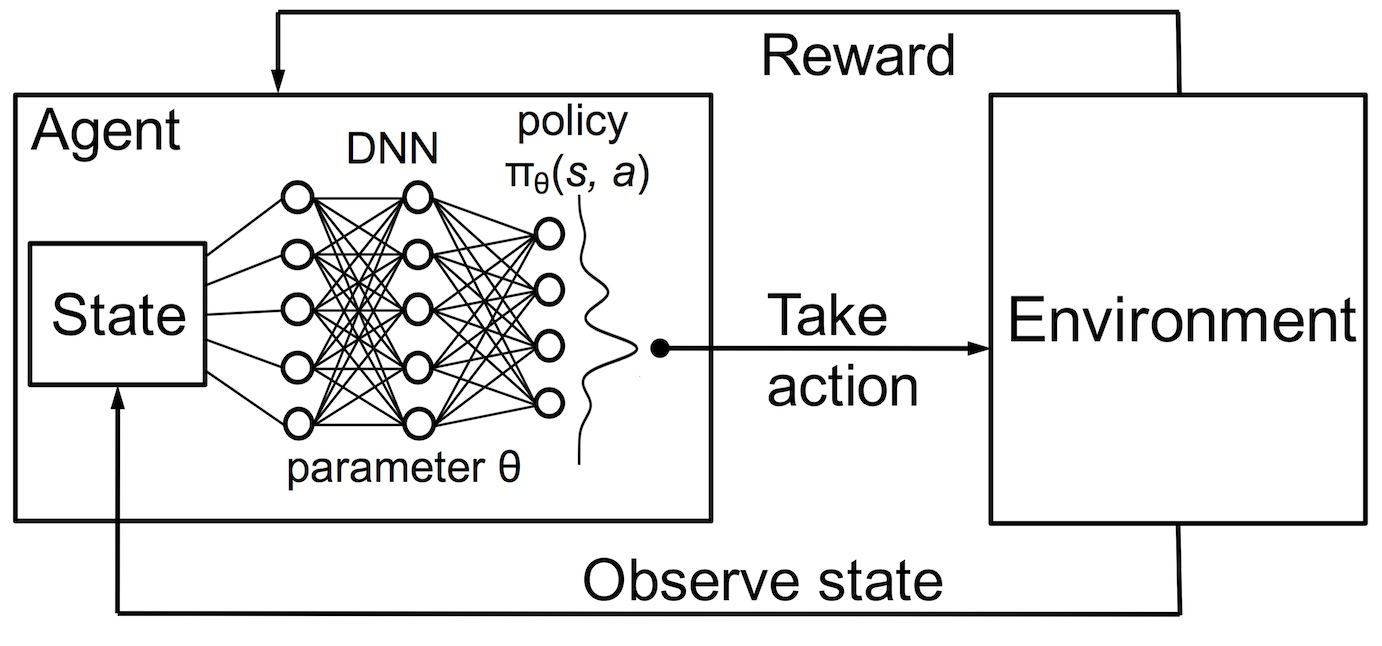
\includegraphics[width=0.5\textwidth]{chapters/chapter2/images/e2e-rl.jpg}
	\caption{Representation of E2E RL models
		\label{fig:e2e-rl}
	}
\end{figure}

\section{DQN on Atari 2600}
\label{bg:sec:dqn}
sdgsdsdfg

\section{CNN Visualisation}
\label{bg:sec:cnn-vis}
sdfsdfsdfsdfsdf